\documentclass[hyperref={pdfpagelabels=false}]{beamer}
\usepackage{lmodern}
\usepackage{amsmath}
\usepackage{graphicx}
%\usepackage{mathptmx} % seems something to do with the font
\usepackage{helvet}
\usepackage{tcolorbox}
\usepackage{lipsum}
\usepackage{textpos}
\usepackage{tikz}

\renewcommand{\familydefault}{helvetica}


\usetheme{Frankfurt}
\setbeamercolor{section in head/foot}{fg=white, bg=blue!20!black!90}


%% commands definitions for
\newcommand\mynew{andyandyandy}

%% end of the definition of commands


%% configuration for the slids style
\makeatletter
\setbeamertemplate{footline}
{
  \leavevmode%
  \hbox{%
    \begin{beamercolorbox}[wd=.333333\paperwidth,ht=2.25ex,dp=1.6ex,center]{author in head/foot}%
      \usebeamerfont{author in
        head/foot}%
      \insertshortauthor\hspace{1em}\beamer@ifempty{Advanced
        Algorithms}{}{Advanced
        Algorithms}
    \end{beamercolorbox}%
    \begin{beamercolorbox}[wd=.333333\paperwidth,ht=2.25ex,dp=1.6ex,center]{title in head/foot}%
      \usebeamerfont{title in head/foot}\insertshorttitle
    \end{beamercolorbox}%
    \begin{beamercolorbox}[wd=.333333\paperwidth,ht=2.25ex,dp=1.6ex,right]{date in head/foot}%
      \usebeamerfont{date in head/foot}\insertshortdate{}\hspace*{2em}
      \insertframenumber{} / \inserttotalframenumber\hspace*{2ex}
    \end{beamercolorbox}}%
  \vskip0pt%
}
\makeatother

\author[\parbox{.2\paperwidth}{}]{Hu SiXing, Hakki Can Karaimer, Pan An, Philipp Keck}
\institute{National University of Singapore}
\title{Convex Optimization}

%% end of configuration



% \title{Convex Optimization}
% \author{Hu SiXing, Hakki Can Karaimer, Pan An, Philipp Keck}
% \date{\today}
\begin{document}

\begin{frame}
  \titlepage
\end{frame}


% \begin{frame}
%   % \frametitle{Table of contents}
%   % \tableofcontents
% %%% Local Variables:
%%% mode: latex
%%% TeX-master: t
%%% End:

%%  commands definition and some other definitions about stuffs
\newcommand\here{lalala}
%\newcommand\x{x_i}
%\newcommand\y{y_i
\newcommand\dis{\displaystyle }


\subsection{}
\begin{frame}
  \frametitle{Linear Regression Example}
  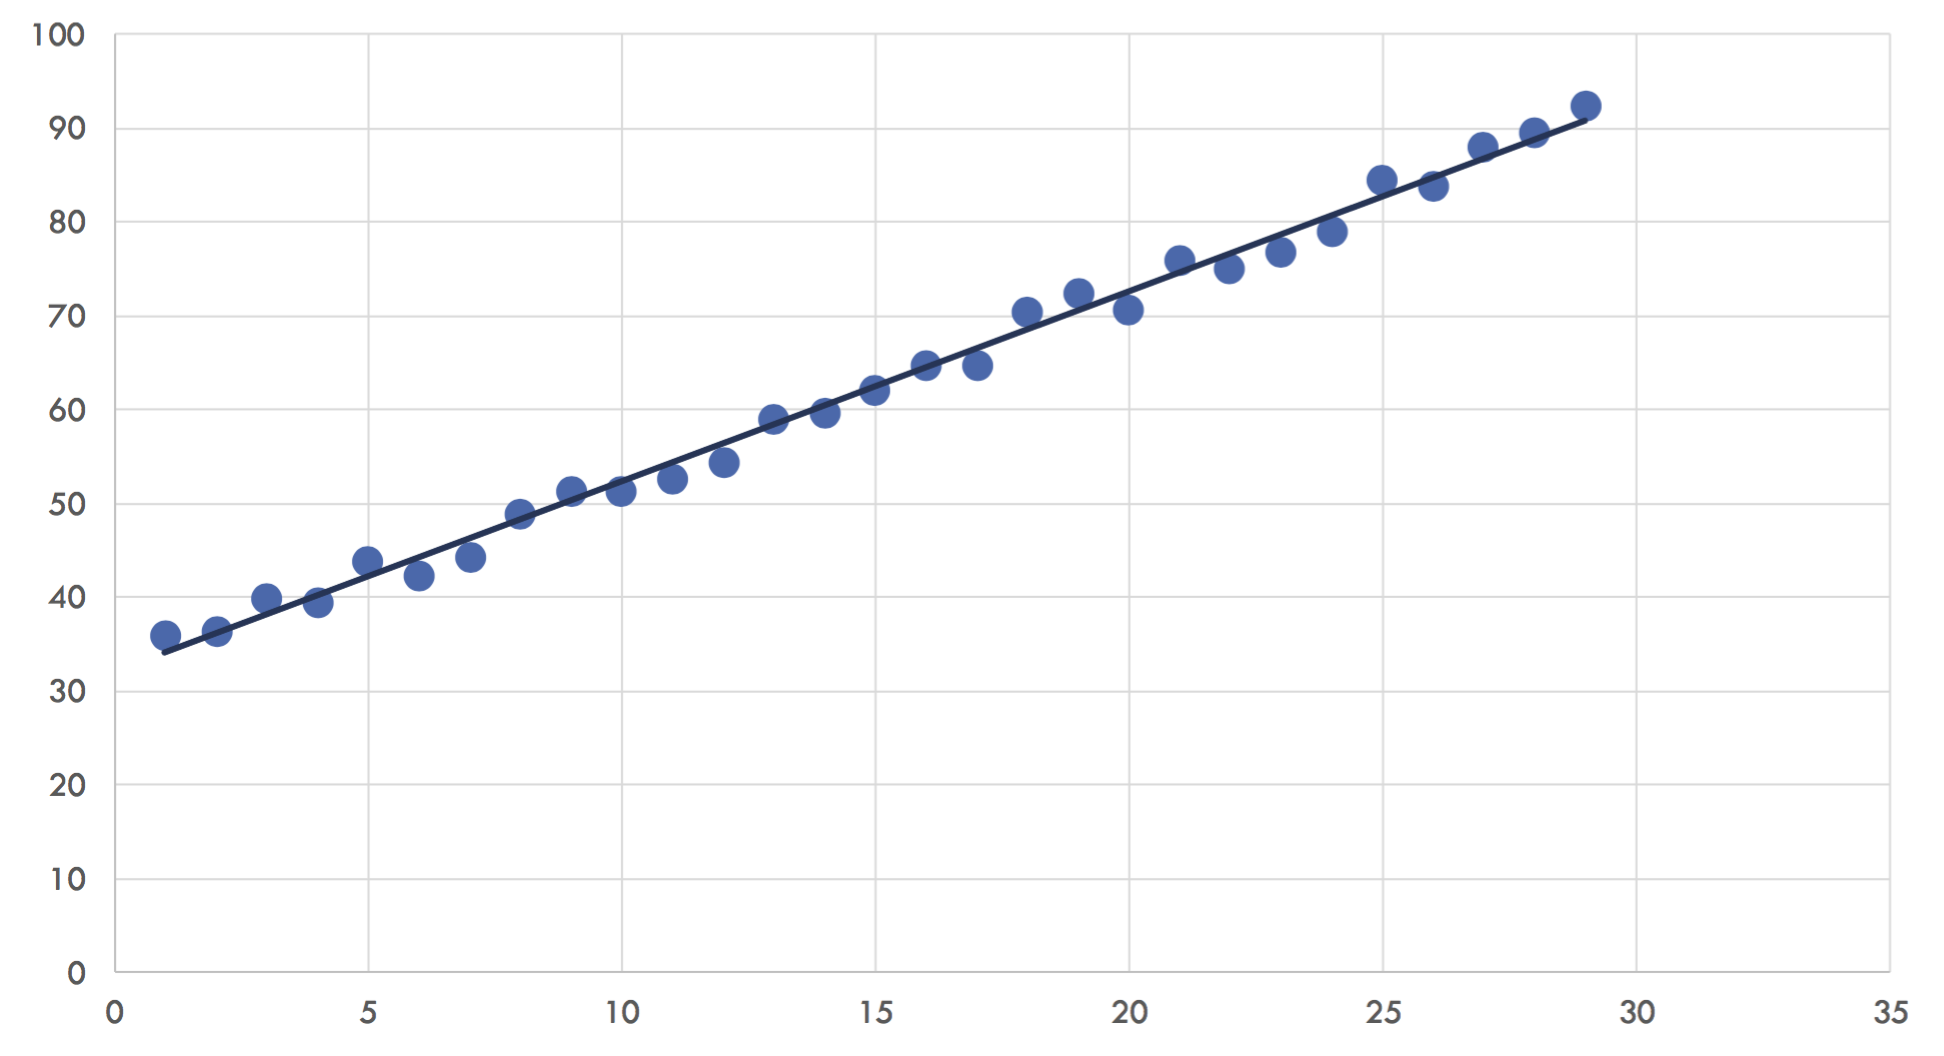
\includegraphics[scale=0.32]{pics/linear.png}

\end{frame}


\subsection{}
\begin{frame}
\frametitle{Ordinary Least Squares}

% 2 columns examples
\begin{columns}
  \begin{column}{0.6\textwidth}
    \begin{itemize}
    \item[] Input: points $(x_i, y_i)$
      \item[] Regression line: $y = mx + b$
\item[] Objective: $\displaystyle \min_{m, b} \sum_{i}(y_i - mx_i -b)^2$
    \end{itemize}
  \end{column}

  \begin{column}{0.5\textwidth}
    \begin{itemize}
    \item[] $(\vec{x_i}, y_i)$
    \item[] $y = \vec{w} \cdot \vec{x} + b$
    \item[] $\dis \min_{\vec{w}}\sum_{i}(y_i - \vec{w} \cdot \vec{x_i} -b)^2$
    \end{itemize}

  \end{column}
\end{columns}

\begin{itemize}
\item Easily Solved: $\vec{w}^*(X^TX)-X^T\vec{y}$
\item But what if $\dim\vec{x} $ is large?
\item What about other similar regressions?
\end{itemize}

\end{frame}

\subsection{}
\begin{frame}
\frametitle{Convex Optimization Problems}


\begin{itemize}
\item OrdinaryLinearRegression: $\dis \min_{\vec{w}}\sum_i(y_i -
  \vec{w} \cdot \vec{x_i})^2$
\item General: $\dis \min_xf(x)$ where $f(x)$ is convex
\item Set $C$ is convex $\Longleftrightarrow \forall x, y\in C, 0\le t
  \le 1: tx +(1 - t)y \in C$
\item Function $f : \mathbb{R}^n \rightarrow \mathbb{R}$ is convex if
  $\dom f$ is convex and $\exists x, y \in \dom f, 0\le t \le 1:$

\end{itemize}

\vspace{-4mm}

{\small
$$f(tx + (1 - t)y) \le tf(x) + (1 - t)f(y)$$
}

\vspace{-4mm}

\begin{columns}
  \begin{column}{0.5\textwidth}

\begin{itemize}
\item Unconstrained.
\end{itemize}

  \end{column}

  \begin{column}{0.5\textwidth}
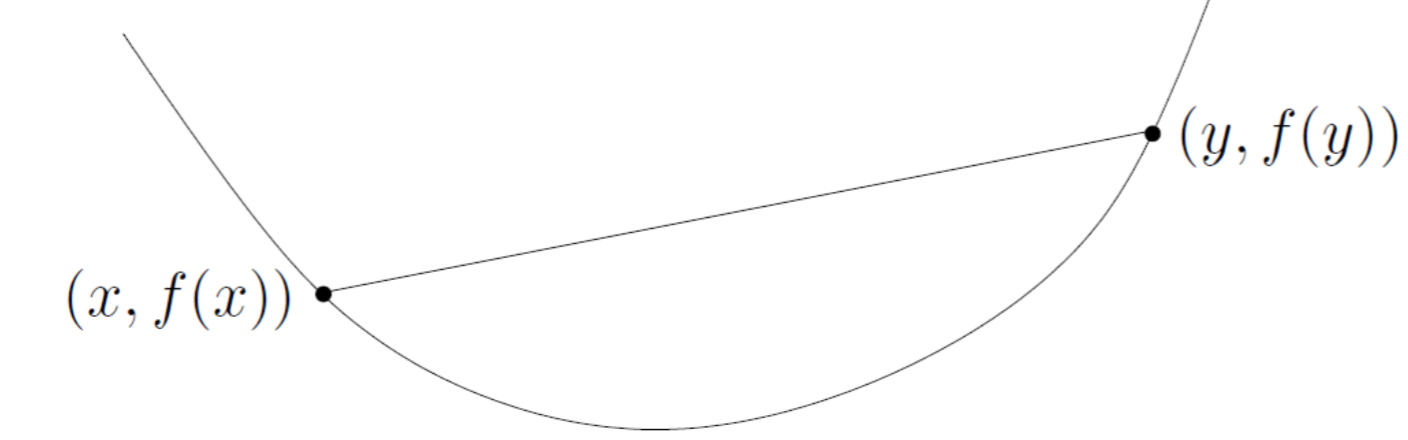
\includegraphics[scale=0.2]{pics/uncons.png}
  \end{column}
\end{columns}

\end{frame}

\subsection{}

\begin{frame}
  \frametitle{Outliers}
  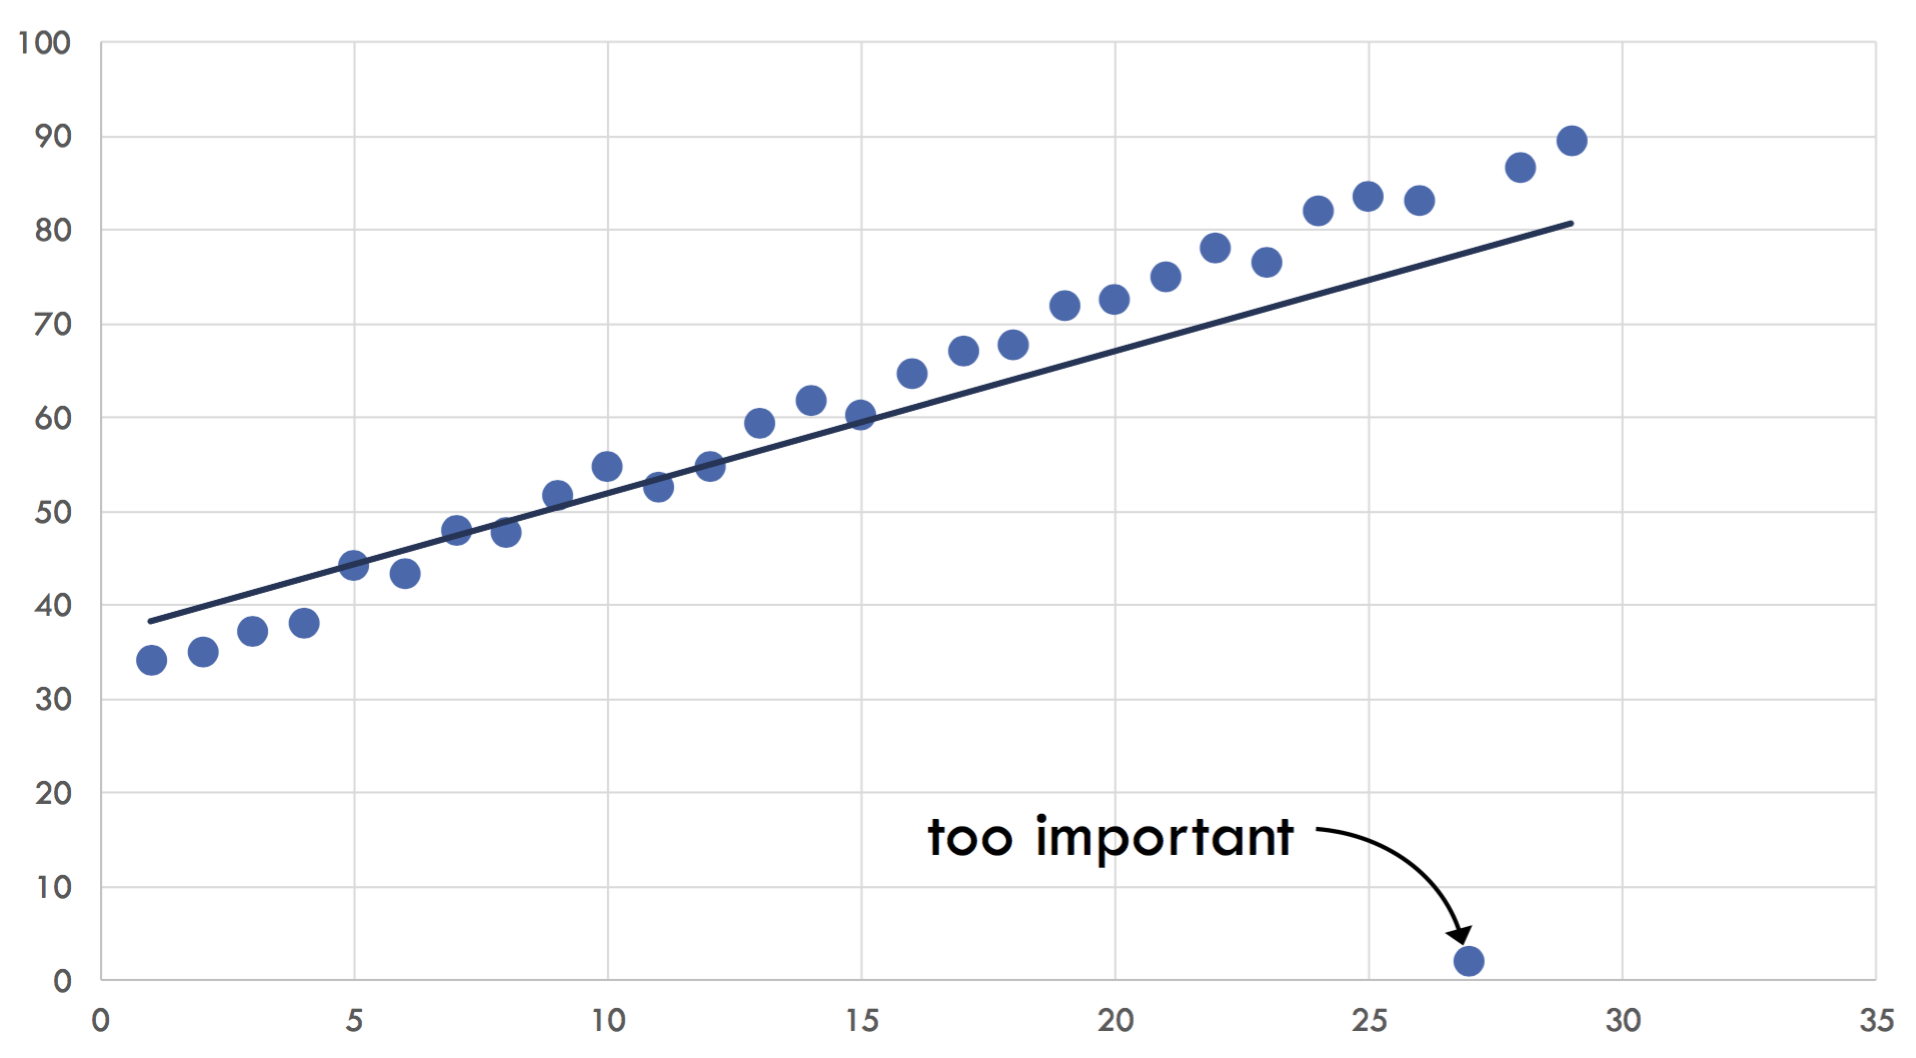
\includegraphics[scale=0.32]{pics/lpo.png}

\end{frame}

\subsection{}
\begin{frame}


  \frametitle{Outlier Penalty}

  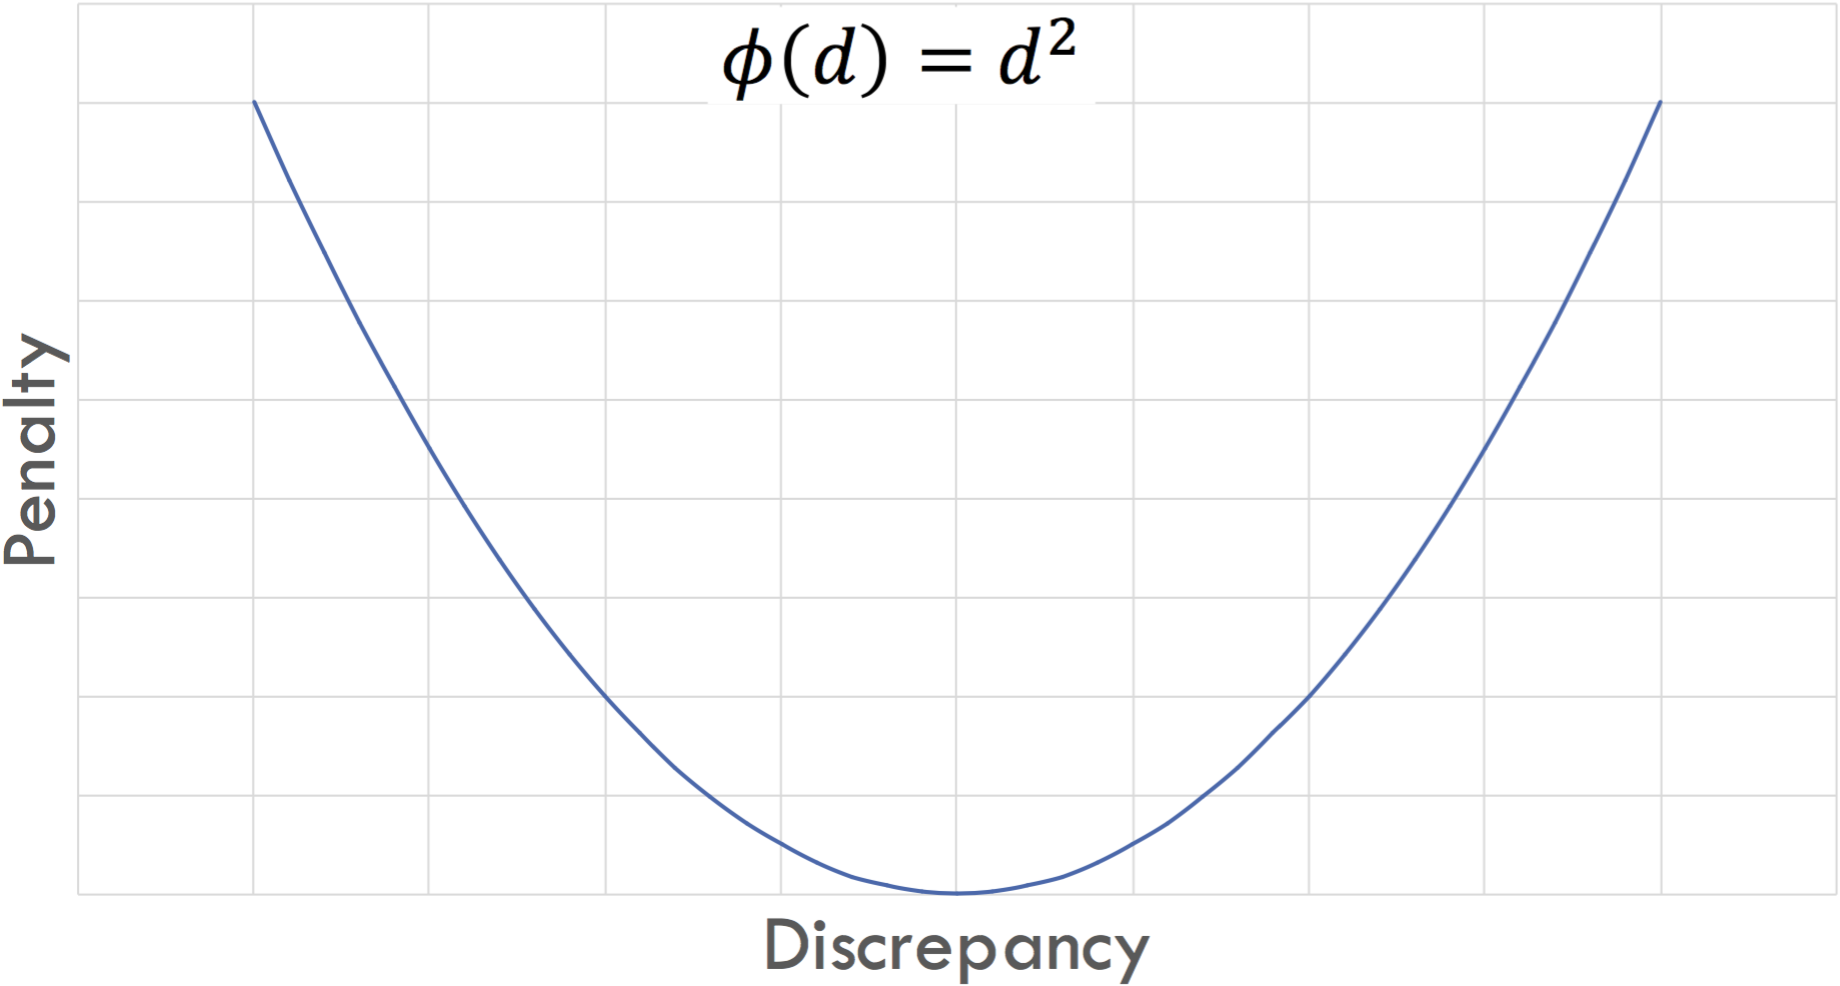
\includegraphics[scale=0.32]{pics/pen1.png}


\end{frame}

\begin{frame}
  \frametitle{Capped Penalty}
  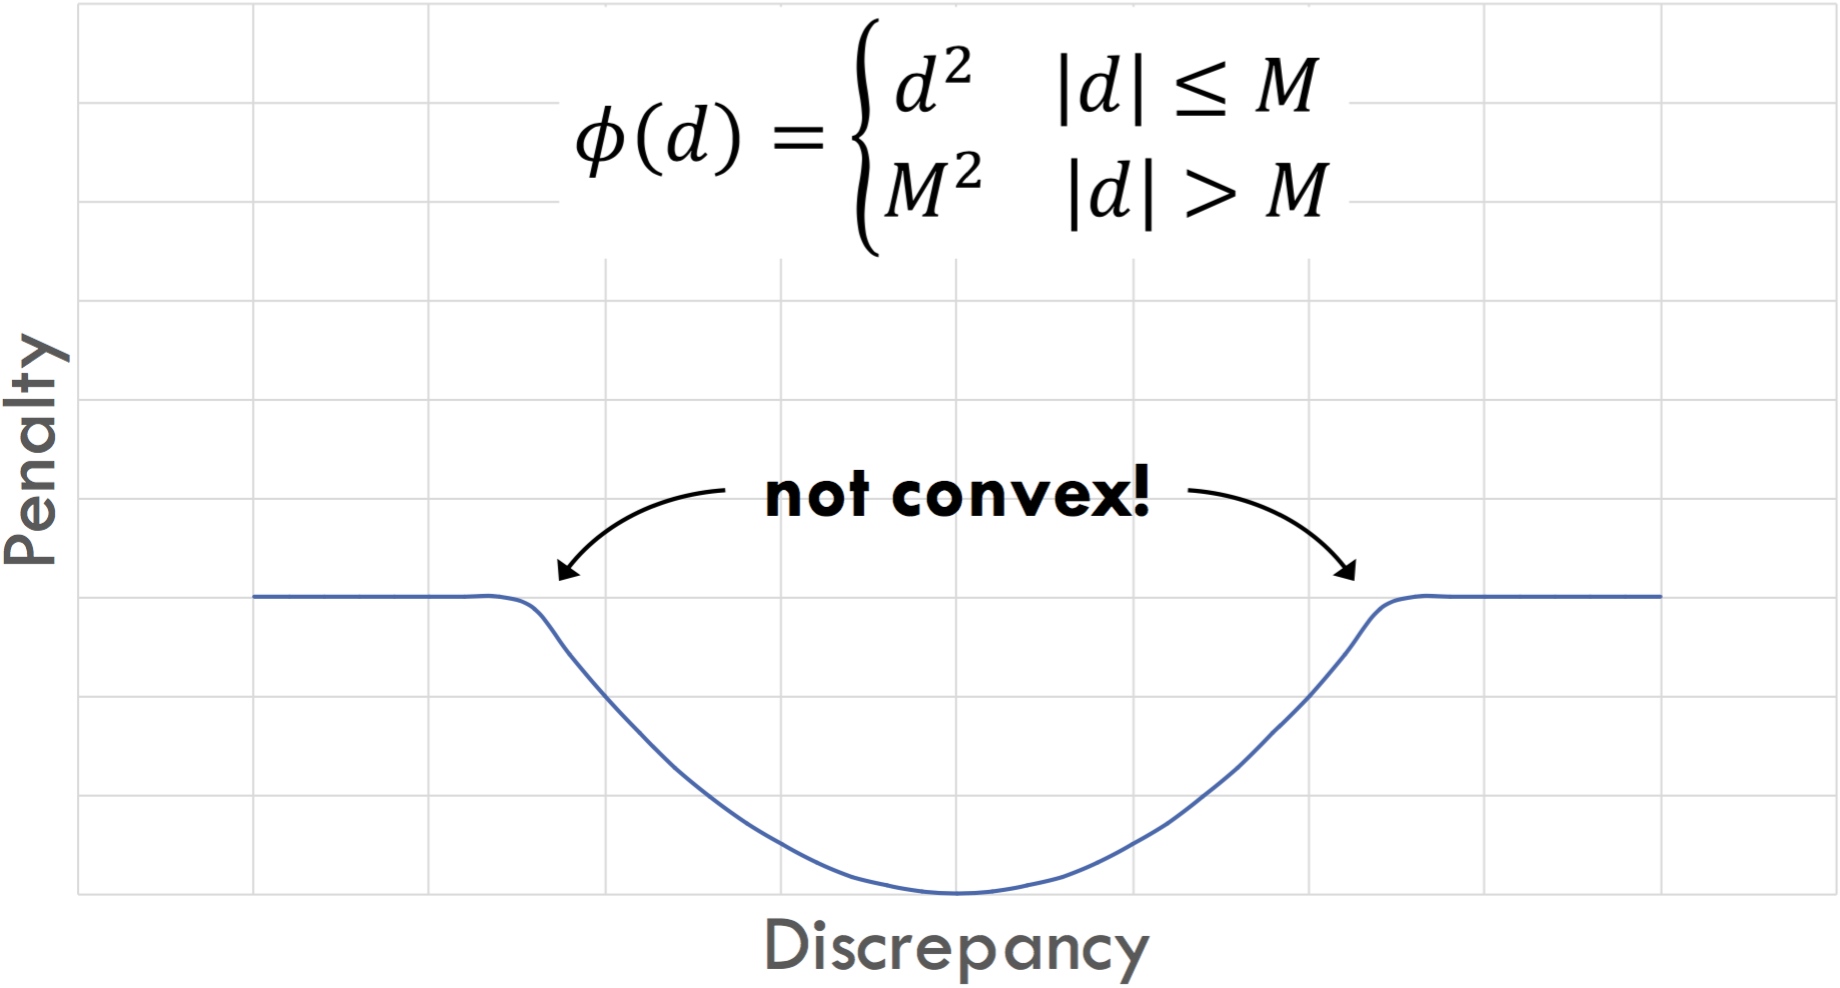
\includegraphics[scale=0.32]{pics/pen2.png}
\end{frame}

\begin{frame}
\frametitle{Huber Penalty Function}
  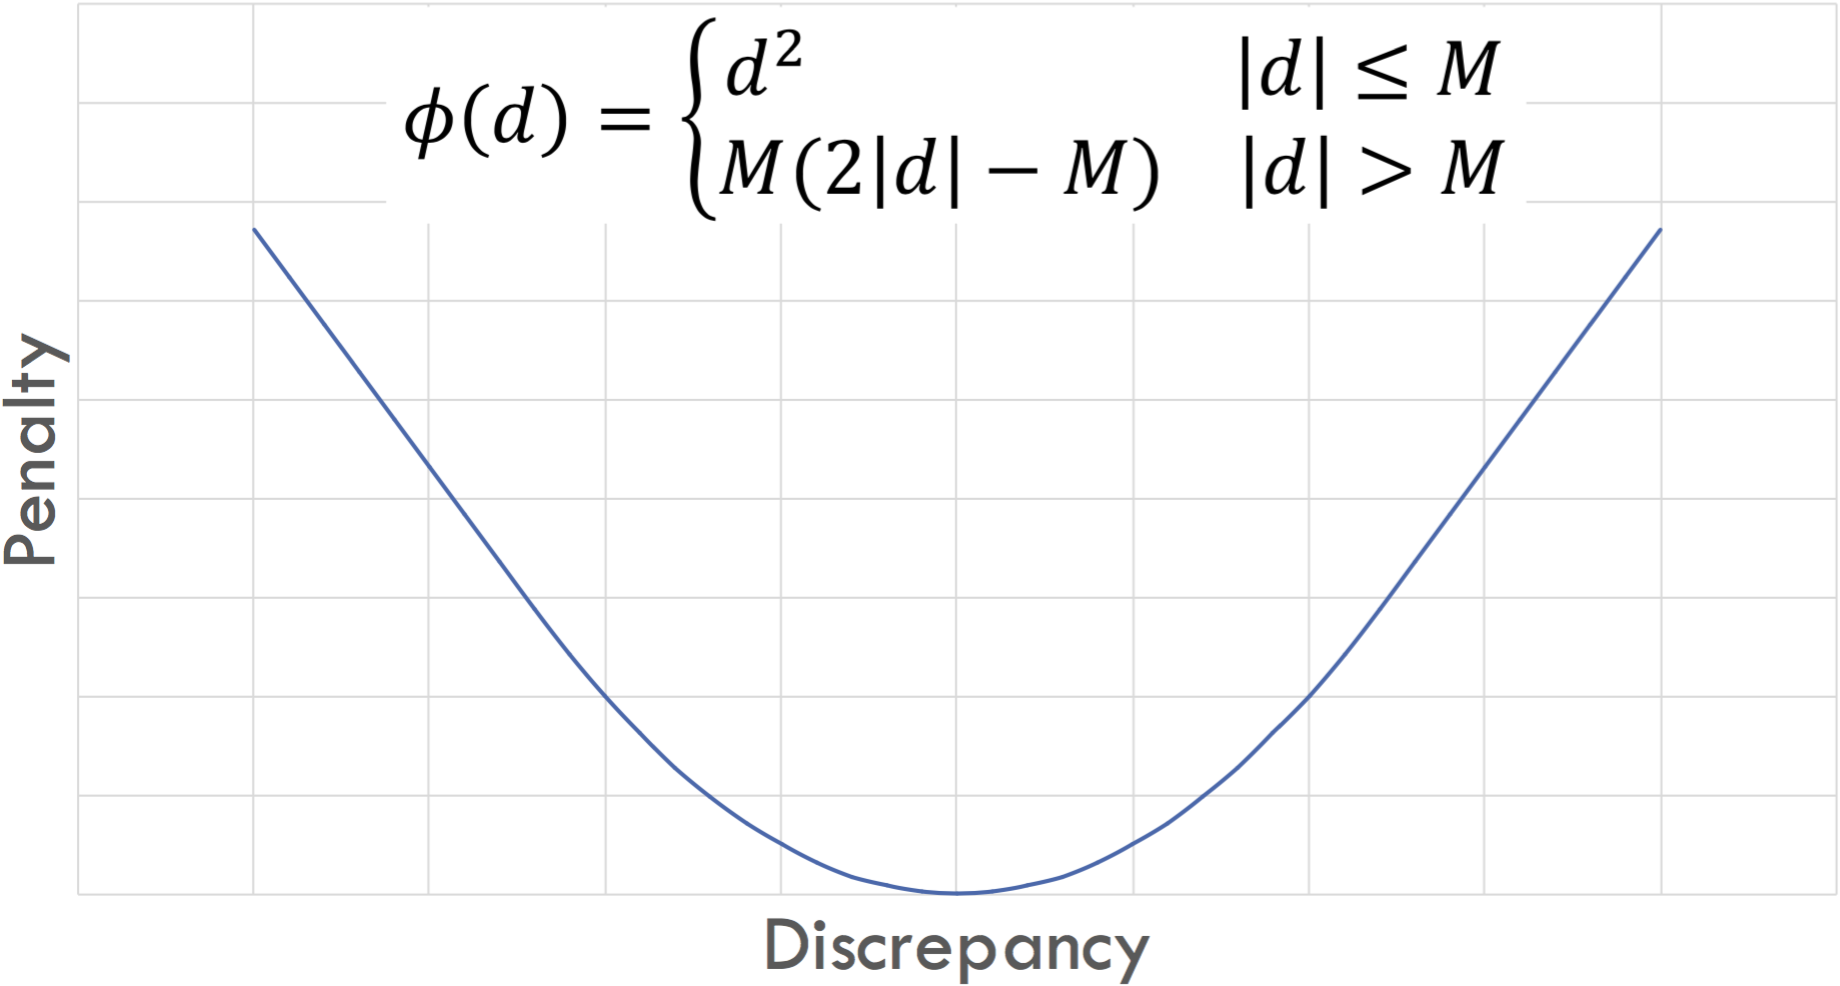
\includegraphics[scale=0.32]{pics/pen3.png}
\end{frame}

% \mynew
% \end{frame}


\section{Linear Regression}
%%% Local Variables:
%%% mode: latex
%%% TeX-master: t
%%% End:

%%  commands definition and some other definitions about stuffs
\newcommand\here{lalala}
%\newcommand\x{x_i}
%\newcommand\y{y_i
\newcommand\dis{\displaystyle }


\subsection{}
\begin{frame}
  \frametitle{Linear Regression Example}
  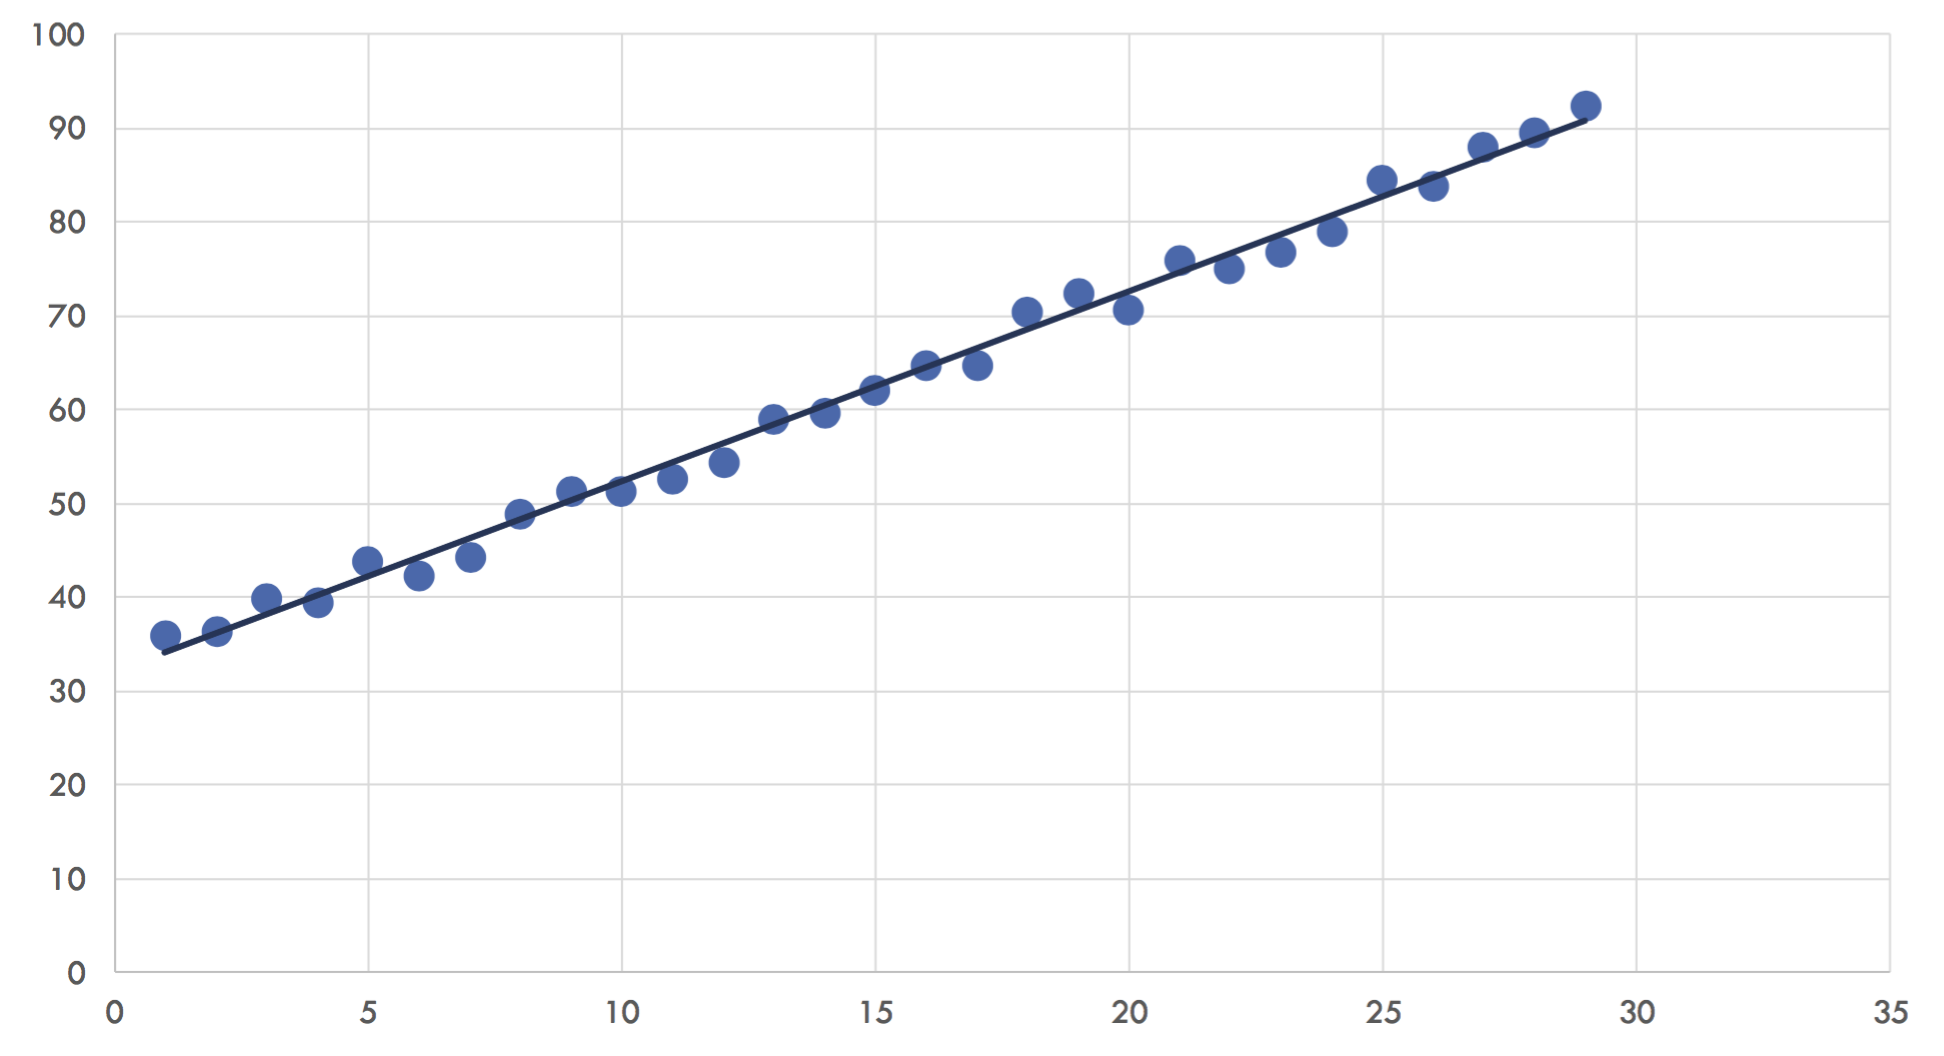
\includegraphics[scale=0.32]{pics/linear.png}

\end{frame}


\subsection{}
\begin{frame}
\frametitle{Ordinary Least Squares}

% 2 columns examples
\begin{columns}
  \begin{column}{0.6\textwidth}
    \begin{itemize}
    \item[] Input: points $(x_i, y_i)$
      \item[] Regression line: $y = mx + b$
\item[] Objective: $\displaystyle \min_{m, b} \sum_{i}(y_i - mx_i -b)^2$
    \end{itemize}
  \end{column}

  \begin{column}{0.5\textwidth}
    \begin{itemize}
    \item[] $(\vec{x_i}, y_i)$
    \item[] $y = \vec{w} \cdot \vec{x} + b$
    \item[] $\dis \min_{\vec{w}}\sum_{i}(y_i - \vec{w} \cdot \vec{x_i} -b)^2$
    \end{itemize}

  \end{column}
\end{columns}

\begin{itemize}
\item Easily Solved: $\vec{w}^*(X^TX)-X^T\vec{y}$
\item But what if $\dim\vec{x} $ is large?
\item What about other similar regressions?
\end{itemize}

\end{frame}

\subsection{}
\begin{frame}
\frametitle{Convex Optimization Problems}


\begin{itemize}
\item OrdinaryLinearRegression: $\dis \min_{\vec{w}}\sum_i(y_i -
  \vec{w} \cdot \vec{x_i})^2$
\item General: $\dis \min_xf(x)$ where $f(x)$ is convex
\item Set $C$ is convex $\Longleftrightarrow \forall x, y\in C, 0\le t
  \le 1: tx +(1 - t)y \in C$
\item Function $f : \mathbb{R}^n \rightarrow \mathbb{R}$ is convex if
  $\dom f$ is convex and $\exists x, y \in \dom f, 0\le t \le 1:$

\end{itemize}

\vspace{-4mm}

{\small
$$f(tx + (1 - t)y) \le tf(x) + (1 - t)f(y)$$
}

\vspace{-4mm}

\begin{columns}
  \begin{column}{0.5\textwidth}

\begin{itemize}
\item Unconstrained.
\end{itemize}

  \end{column}

  \begin{column}{0.5\textwidth}
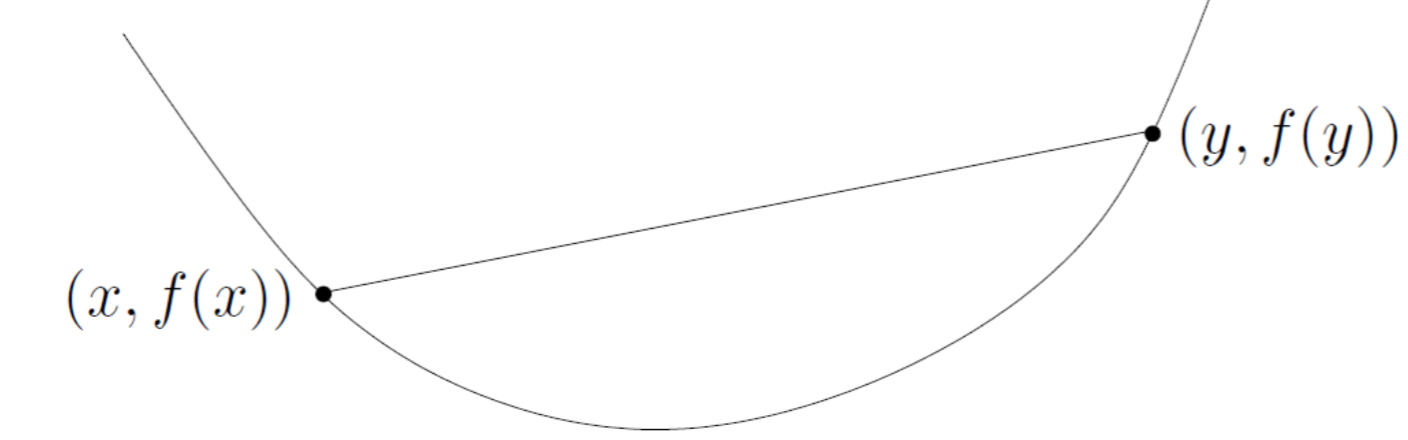
\includegraphics[scale=0.2]{pics/uncons.png}
  \end{column}
\end{columns}

\end{frame}

\subsection{}

\begin{frame}
  \frametitle{Outliers}
  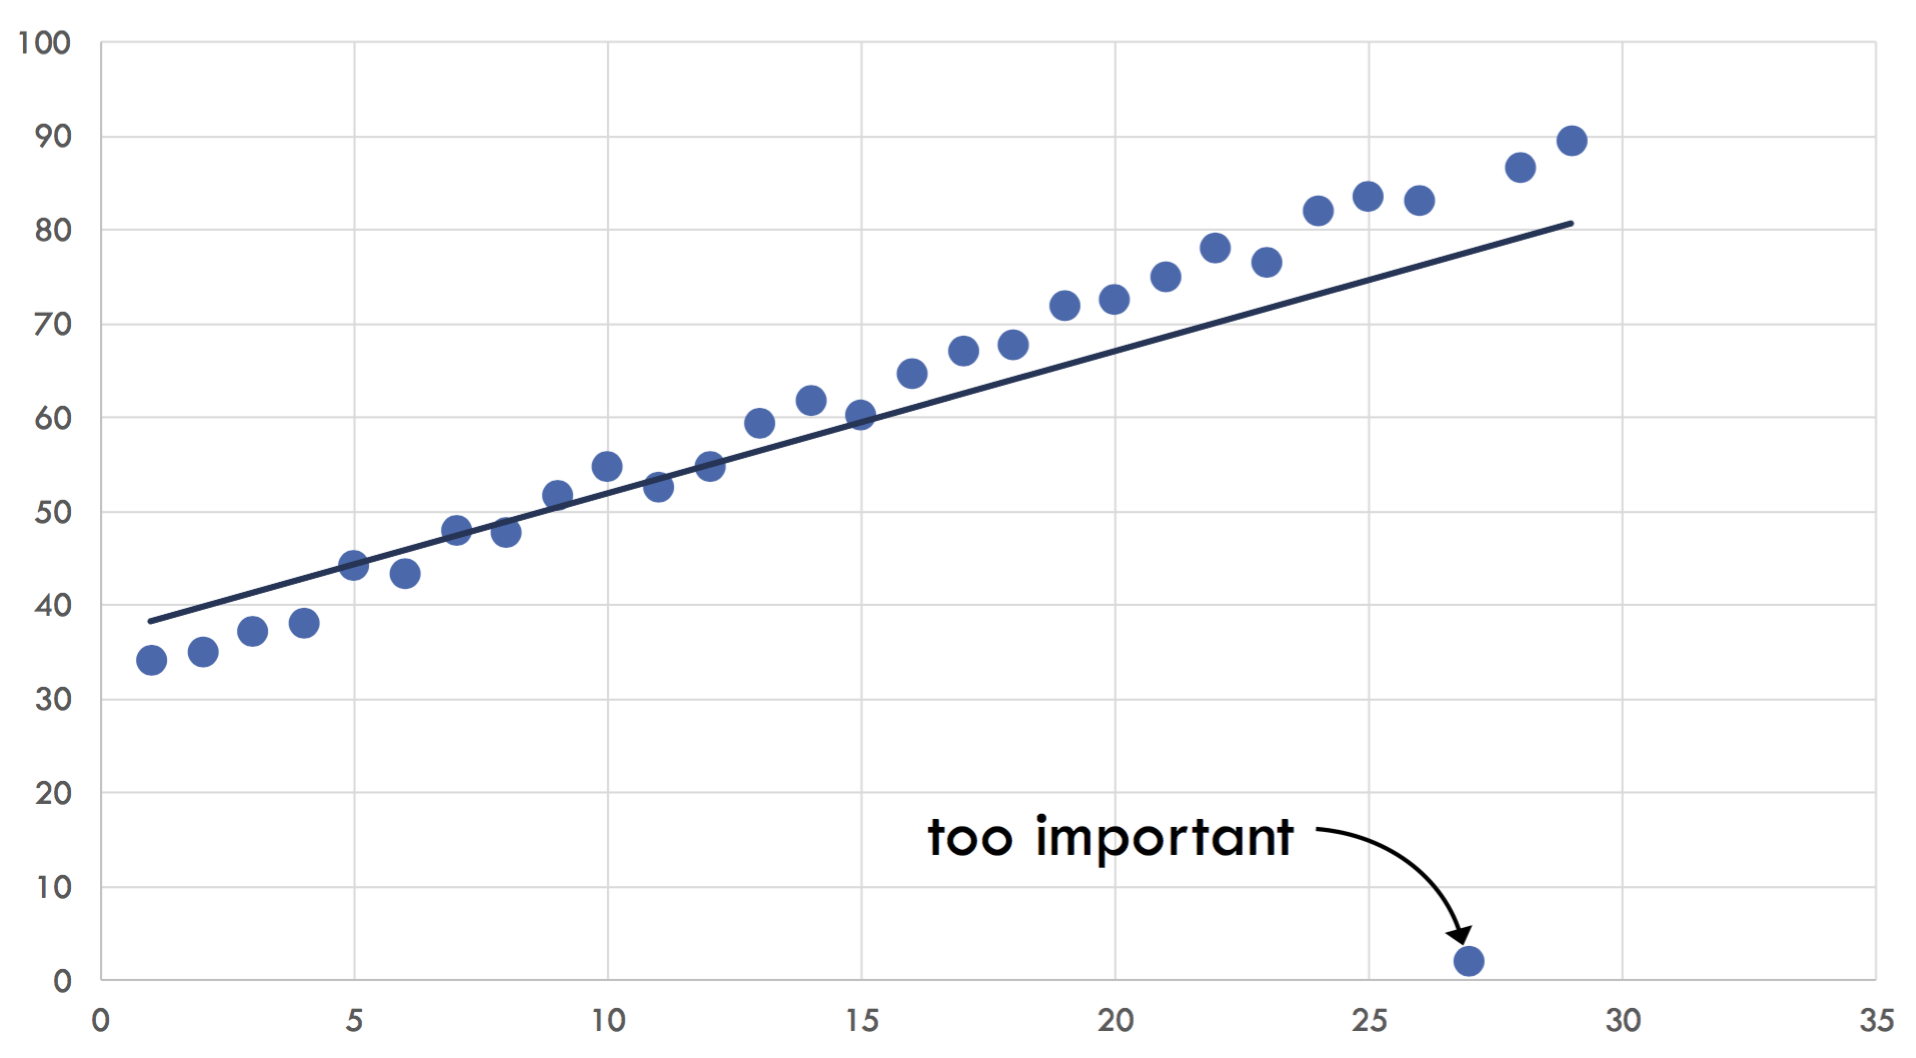
\includegraphics[scale=0.32]{pics/lpo.png}

\end{frame}

\subsection{}
\begin{frame}


  \frametitle{Outlier Penalty}

  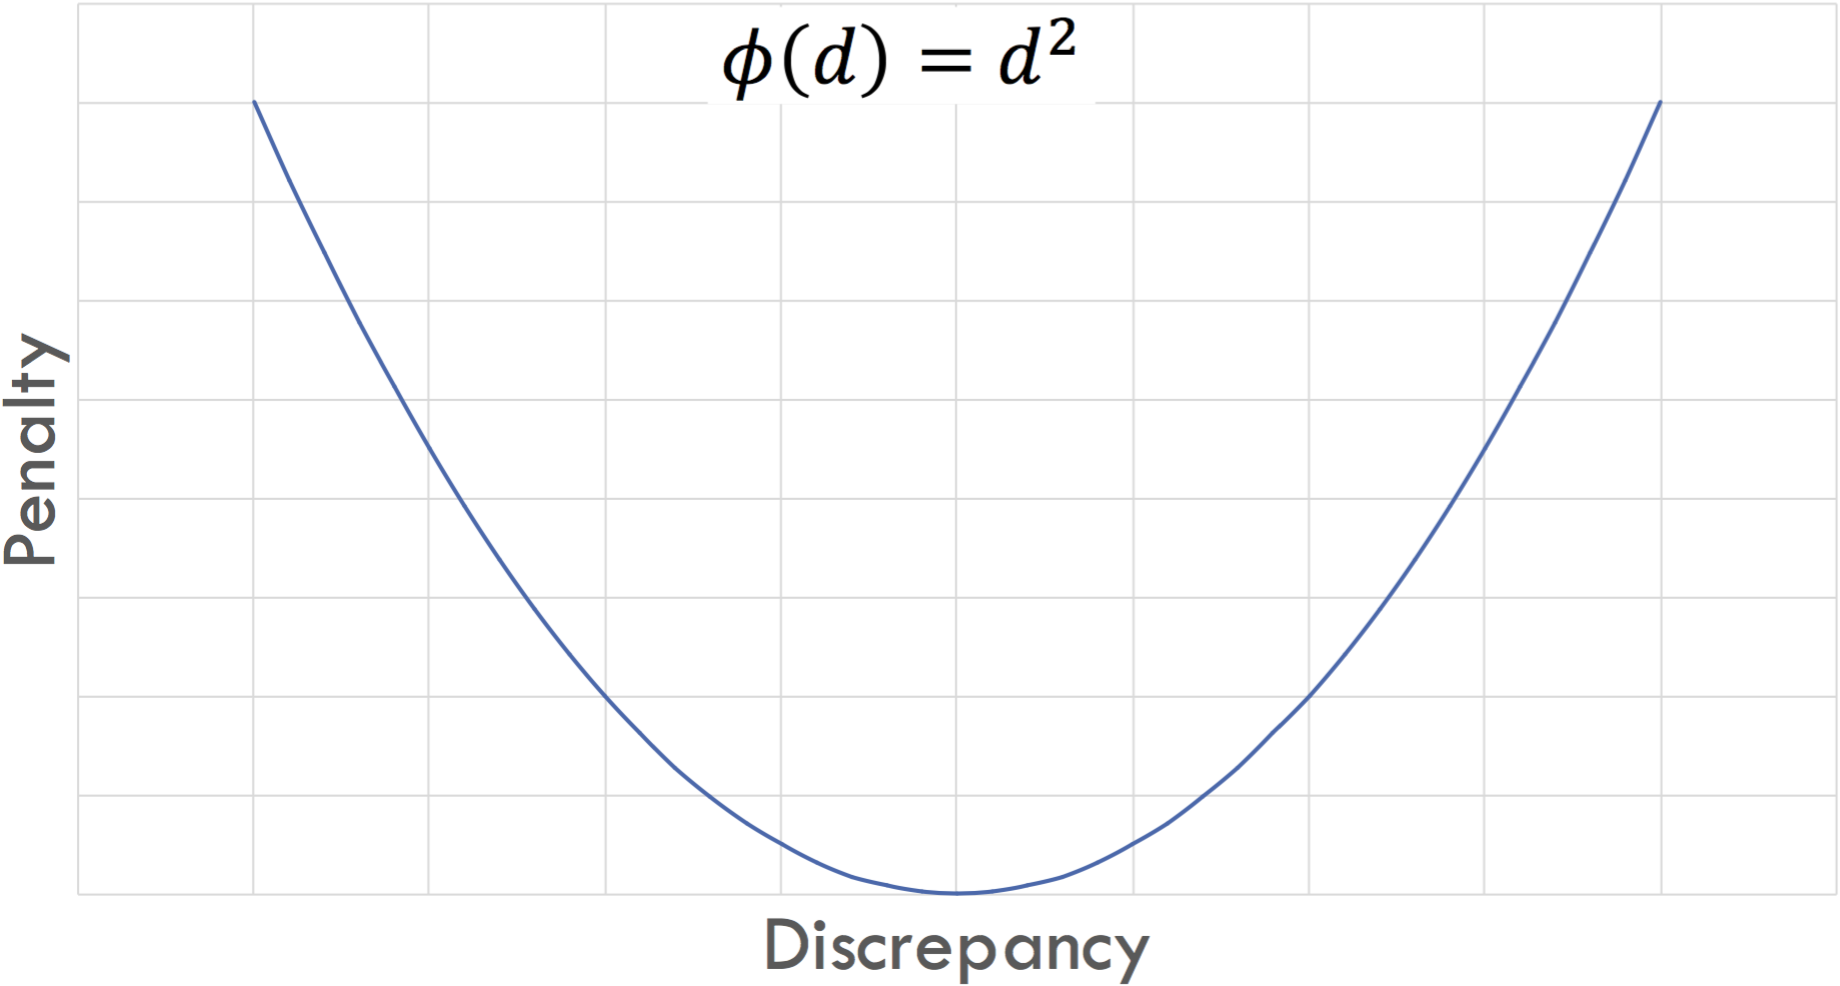
\includegraphics[scale=0.32]{pics/pen1.png}


\end{frame}

\begin{frame}
  \frametitle{Capped Penalty}
  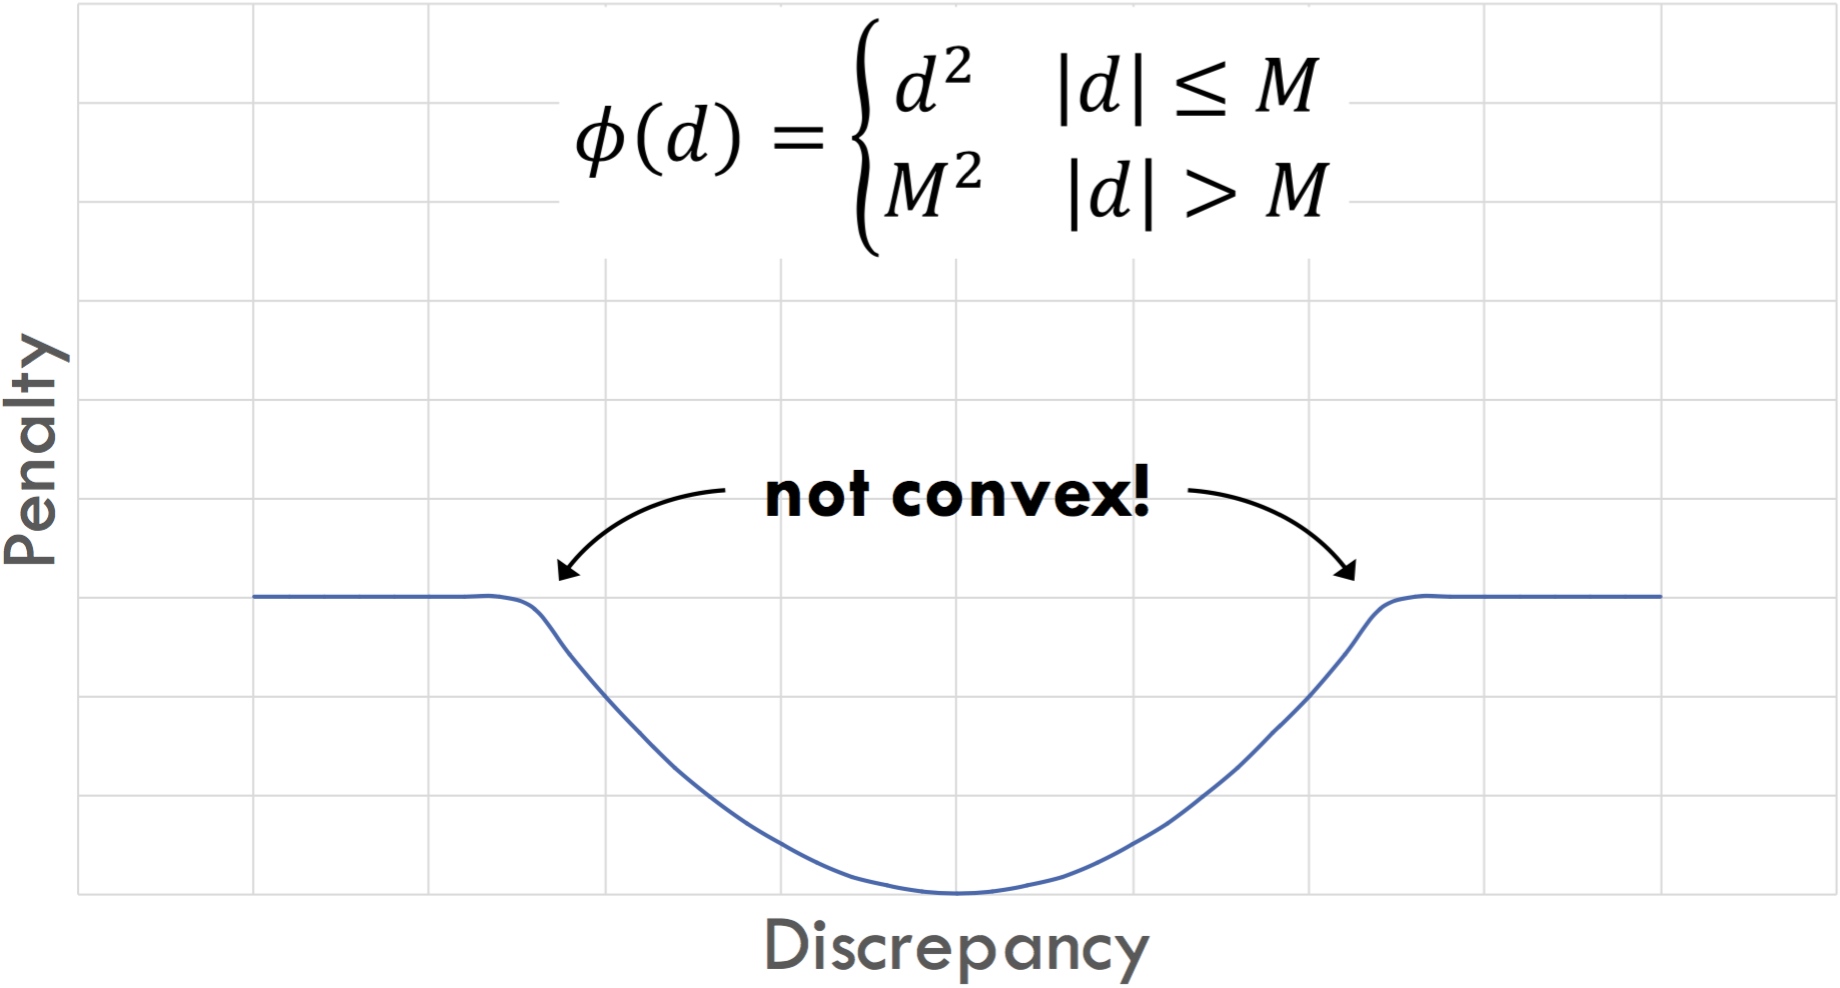
\includegraphics[scale=0.32]{pics/pen2.png}
\end{frame}

\begin{frame}
\frametitle{Huber Penalty Function}
  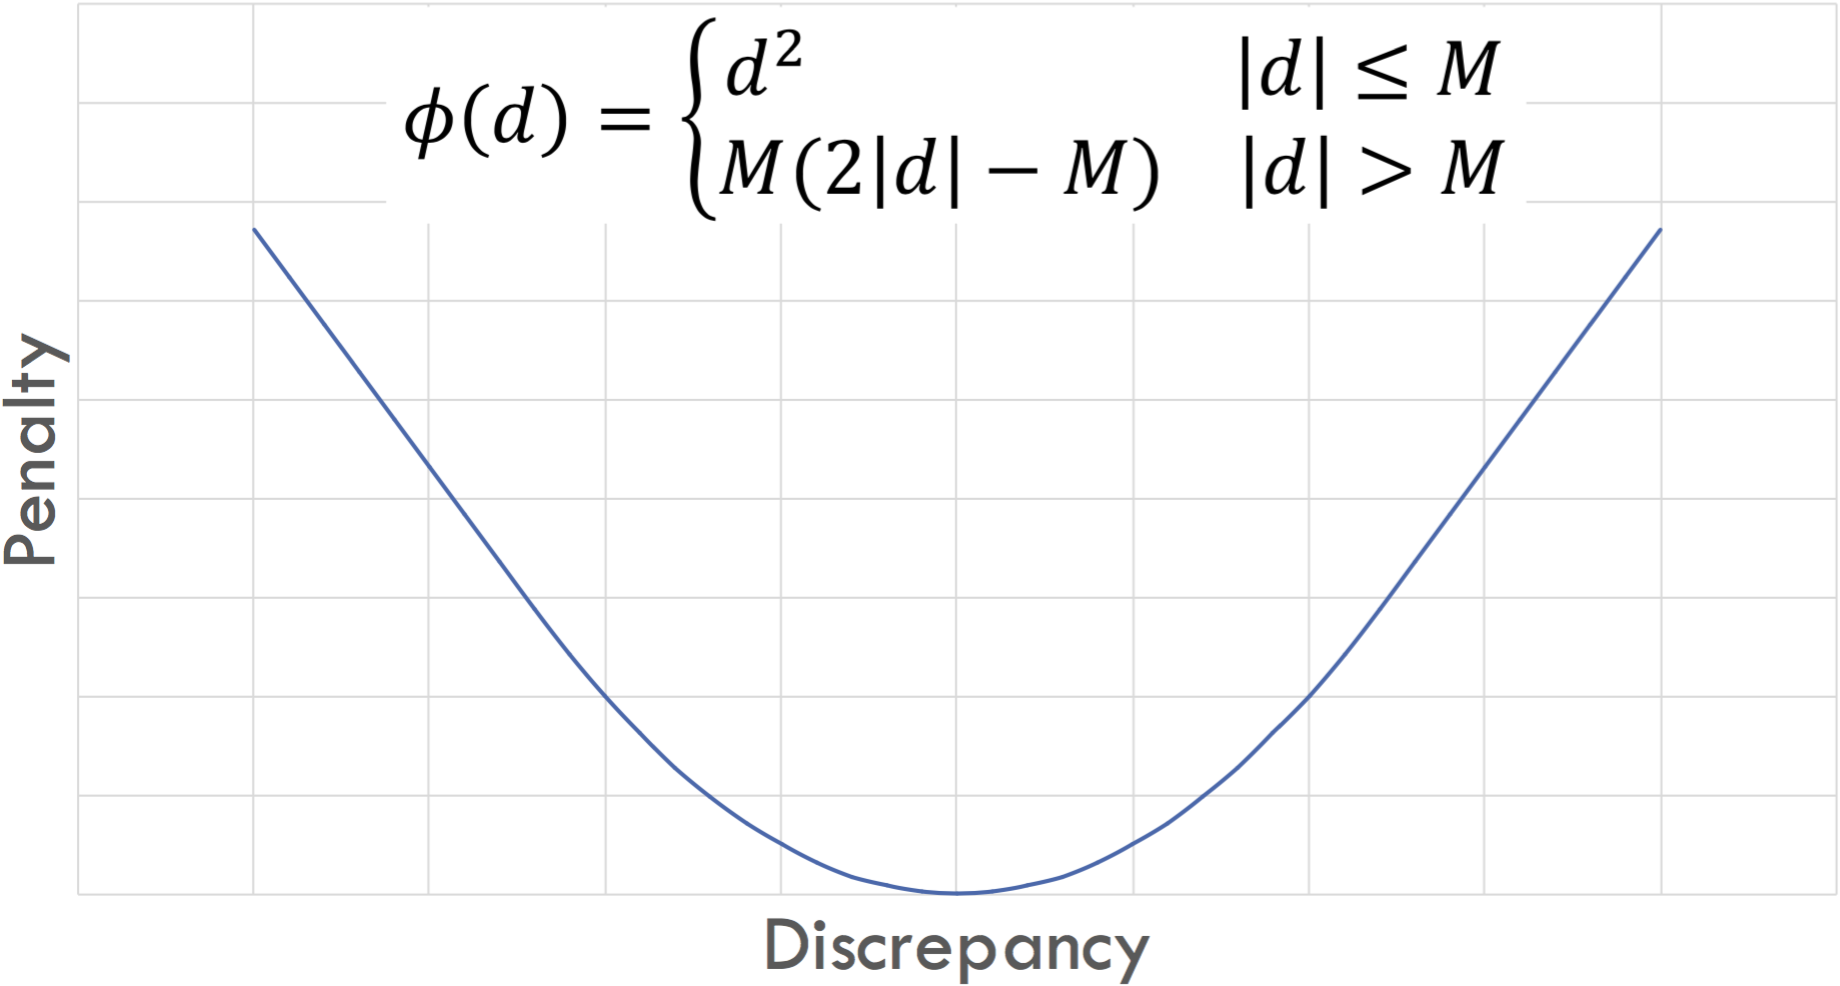
\includegraphics[scale=0.32]{pics/pen3.png}
\end{frame}


\section{Applications}
%%% Local Variables:
%%% mode: latex
%%% TeX-master: t
%%% End:

\newenvironment<>{redblock}[1]{%
  \setbeamercolor{block title}{fg=white,bg=red!75!black!65}%
  \setbeamercolor{block body}{fg=red!40!black!70,bg=red!60!black!20}%

  \begin{block}#2{#1}}{\end{block}}
\newenvironment<>{blueblock}[1]{%
  \setbeamercolor{block title}{fg=white,bg=blue!75!black!65}%
  \setbeamercolor{block body}{fg=black,bg=blue!60!black!20}%
  \begin{block}#2{#1}}{\end{block}}

\newenvironment<>{greyblock}[1]{%
  \setbeamercolor{block title}{fg=white,bg=black!75}%
  \setbeamercolor{block body}{fg=black,bg=black!40}%
  \begin{block}#2{#1}}{\end{block}}


\section{Applications}

\subsection{Image Processing}

\begin{frame}
\frametitle{Image Processing --- Lucas-Kanade}
  \begin{itemize}
  \item[] {
Classic examples are optical flow techniques like Lucas-Kanade (VideoTracking), Horn-Schunck.
  }
  \end{itemize}


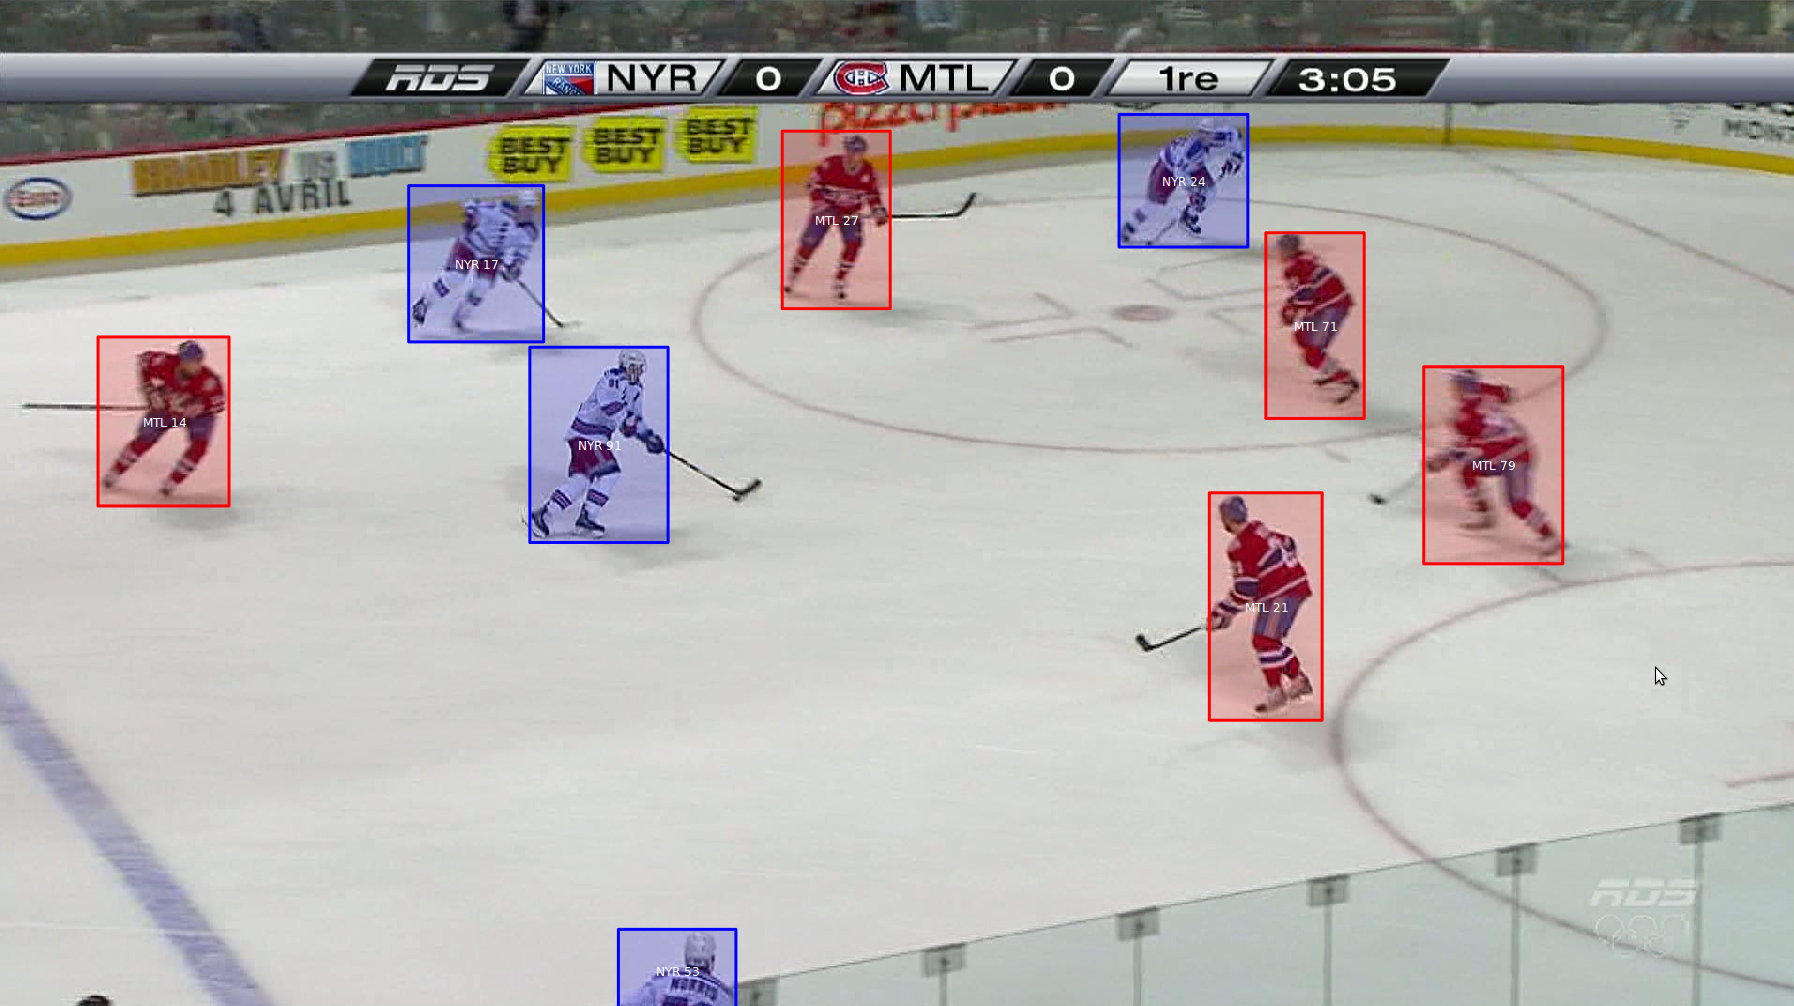
\includegraphics[scale=0.15]{right2.png}
\end{frame}

\begin{frame}
\frametitle{Lucas-Kanade}

\begin{blueblock}{Goal of Lucas-Kanade}
Minimize the sum of squared error between two images.
\end{blueblock}

\begin{redblock}{Assumption}
The displacement of the image contents between two nearby instants
(frames) is small and approximately constant within a neighborhood of
the point $p$ under consideration.
\end{redblock}

\end{frame}

\begin{frame}
\frametitle{Lucas-Kanade}
  \begin{blueblock}{Optical Flow Equation (2 Dementional)}
For a pixel location $(x, y, t)$, the intensity has moved by $\Delta
x, \Delta y, \Delta t$, the basic assumption can be represented as:
$$I(x, y, t) = I(x + \Delta x, y + \Delta y, t + \Delta t)$$

  \end{blueblock}
\end{frame}

\begin{frame}
\frametitle{Lucas-Kanade}
  \begin{blueblock}{Optical Flow Effect:}
For all pixels within a window centered at p:
$$I_x(q_i)V_x + I_y(q_i)V_y = -I_t(q_i) $$
Where  $i = 1,2,3 ... n$.

  \end{blueblock}

  \begin{greyblock}{Abbreviations:}
$$ A = [ I_x(q_i)^T, I_y(qi)^T] $$
$$ V = [v_x, v_y]^T $$
$$ b = [-I_t(q_i)]^T $$
  \end{greyblock}
\end{frame}

\begin{frame}
\frametitle{Lucas-Kanade}
  \begin{blueblock}{Lucas-Kanade Method Abstraction:}
LK method tries to solve $2 \times 2$ system:
$$A^TAV = A^Tb$$

A.K.A:

$$V = (A^TA)^{-1}A^Tb$$
  \end{blueblock}

  \begin{greyblock}{Notice:}
    $V = [v_x, v_y]^T$ is variable. Which means that the system does
    not know the actual velocity of the system.
  \end{greyblock}
\end{frame}


\begin{frame}
\frametitle{Lucas-Kanade}
  \begin{blueblock}{Goal of Lucas-Kanade Method:}
To minimize $||A^TV - b||^2$.
  \end{blueblock}
Basic LK Derivation for Models(Stuff to be Tracked):
$$E[v_x, v_y] = \Sigma [I(x+v_x, y+v_y) - T(x, y)]^2$$
Where $v_x, v_y$ is the hypothesized location of the model(s) to be
tracked, and $T(x, y)$ model.
\end{frame}

\begin{frame}{ \LARGE APPLICATIONS -- IMAGE PROCESSING}
\frametitle{Lucas-Kanade}
  \begin{redblock}{Key Step for Implementation of GD (Step 1):}
    Generalizing LK approach by introducing warp function W:
    $$E[v_x, v_y]  = \Sigma [I(W(x, y); P) - T(x,y)]^2$$
    Generalizing is used to solve the problem where the constant flow
    of larger picture frames for a long time is a total waste of
    calculation power. Warp function examples are {\bf Affine}  and
    {\bf Projective}. \\
The warping function are the {\bf convergence factor} for steepest descent
algorithm.
  \end{redblock}
\end{frame}


\begin{frame}
\frametitle{Lucas-Kanade}
  \begin{redblock}{Key Step for Implementation of GD (Step 2):}
The key to the derivation is Taylor series approximation:
$$ I(W(x, y); P + \Delta P) \approx I(W([x, y]; P)) + \nabla I
\frac{\partial W}{\partial P}\Delta P$$
  \end{redblock}

\begin{itemize}
\item The approximation equation is actually the abstract of the basic
assumption of optical flow described in the slides before.
\item Derivation of this equation can be discussed in forum (Too long
  for slides).

\end{itemize}




\end{frame}

\begin{frame}
\frametitle{Lucas-Kanade}
  \begin{blueblock}{Some Explainations:}
    \begin{itemize}
\item Gradient image $\nabla I$
\item Image error $I_E = T(x, y) - I(W[x, y]; P)$
\item Jacobian matrix $ \frac{\partial W}{\partial P} $
\item Steepest image  $ I_S =  \nabla I \frac{\partial W}{\partial P}$
\item Hessian Matrix $\Sigma (\nabla I \frac{\partial W}{\partial
    P})^T(\nabla I \frac{\partial W}{\partial P})$
\item Iteration step $ \Delta P =  \Sigma I_S^T I_E$
    \end{itemize}

\end{blueblock}

\end{frame}

\begin{frame}
\frametitle{Lucas-Kanade}
  \begin{greyblock}{Algorithms: }
    \begin{itemize}
    \item Warp image and get $I(W[x, y]; P)$;
    \item Get image error $I_E$;
    \item Warp gradient image $\nabla I$;
    \item Evaluate Jacobian;
    \item Compute steepest descent image  $I_S = \nabla I \frac{\partial W}{\partial
    P}$;
    \item Compute Hessian matrix $\Sigma I_S^TI_S$;
    \item Get warping step $\Delta P = I_SI_E$;
    \item Update warping parameter $P = P + \Delta P$;
      \item Repeat until $\Delta P$ is negligible.
    \end{itemize}
  \end{greyblock}
\end{frame}


\subsection{MACHINE LEARNING}


\begin{frame}{ \LARGE APPLICATIONS -- MACHINE LEARNING}
  \begin{blueblock}{Generalized Utilization of Convex: Delta Rule}
\begin{itemize}
\item The delta rule is derived by attempting to minimize the error in the output of the neural network through gradient descent.
\item Gradient Descent optimization is the most basic principle for
  training neurons even with different activation functions.
\item Delta rule, can also be modified, if possible, with steepest descent method.
\end{itemize}
  \end{blueblock}

\end{frame}

\begin{frame}{ \LARGE APPLICATIONS -- MACHINE LEARNING}
  \begin{redblock}{Delta Rule:}
$$\Delta w_{ji} = \alpha (t_j - y_j)g'(h_j)x_j$$
Where $\alpha$ is the learning rate, $g(x)$ is the neuron's activation
function. $t_j$ and $y_j$ is the target and actual output of the
neuron. $h_j$ is the weighted sum of the neuron's inputs. And $x_i$ is
the $i_{th}$ input.
  \end{redblock}

  \begin{greyblock}{The above equation holds the following:}
$$h_j = \Sigma x_iw_{ji}$$
$$y_j = g(h_j)$$

  \end{greyblock}

\end{frame}

\subsection{ROBOTICS}
\begin{frame}{ \LARGE APPLICATIONS -- INVERSE KINEMATICS}
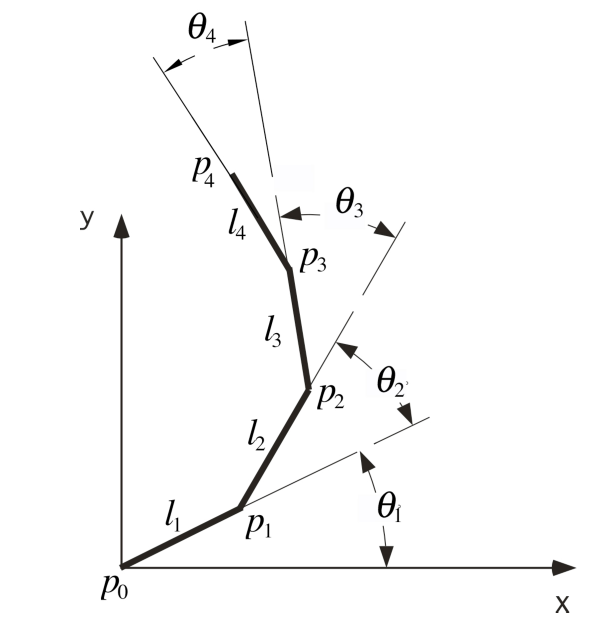
\includegraphics[scale=0.6]{jcob.png}

\end{frame}

\begin{frame}{ \LARGE APPLICATIONS -- INVERSE KINEMATICS}
  \begin{blueblock}{Goal of Inverse Kinematics}
Given a position in the space, calculate a way for a robot hand to reach a place.

  \end{blueblock}
  \begin{redblock}{Problem Abstract:}
$$\vec{e} = R_1T_1R_2T_2R_3T_3R_4T_4\vec{e_0}$$
 Where $T_i$ is a series of translation transformation and $R_i$ is a
 series of rotation translation.

  \end{redblock}

\end{frame}

\begin{frame}{ \LARGE APPLICATIONS -- INVERSE KINEMATICS}
  \begin{redblock}{Abstraction for Convex Optimization:}
$$\Delta \vec{\theta} = \alpha J^T \vec{e}$$.

The target for the optimization is to achieve $|\vec{e_p}-\vec{e_t}| =
0$, where $\vec{e_p}$ is th original position of the tip of the
robotic arm and $\vec{e_t}$ is the target position.
$J$ is the jacobian matrix in terms of $\vec{\theta}$, which is the
vector of all the spatial angles of all  joints. $\alpha$ is the
convergence rate and $\vec{e}$ is the position derivation (step size).

  \end{redblock}

\end{frame}

\begin{frame}{ \LARGE APPLICATIONS -- INVERSE KINEMATICS}
  \begin{greyblock}{About Inverse Kinematics}
    \begin{itemize}
    \item Jacobian transpose is the implementation of gradient descent
      in the real physical world.
    \item It can actually achieve {\bf near linear} solution for
      robotic arms with a fast convergence rate.
    \end{itemize}
  \end{greyblock}

\end{frame}



% \section{Section no. 2}
% \subsection{Lists I}
% \begin{frame}
%   \frametitle{unnumbered lists}
%   \begin{itemize}
%   \item Introduction to  \LaTeX{}
%   \item Course 2
%   \item Termpapers and presentations with \LaTeX{}
%   \item Beamer class
%   \end{itemize}
% \end{frame}

% \begin{frame}\frametitle{lists with single pauses}
%   \begin{itemize}
%   \item Introduction to  \LaTeX{}  \pause
%   \item Course 2 \pause
%   \item Termpapers and presentations with \LaTeX{}  \pause
%   \item Beamer class
%   \end{itemize}
% \end{frame}

% \begin{frame}\frametitle{lists with pause}
%   \begin{itemize}[<+->]
%   \item Introduction to  \LaTeX{}
%   \item Course 2
%   \item Termpapers and presentations with \LaTeX{}
%   \item Beamer class
%   \end{itemize}
% \end{frame}



% \subsection{Lists II}
% \begin{frame}\frametitle{numbered lists}
%   \begin{enumerate}
%   \item Introduction to  \LaTeX{}
%   \item Course 2
%   \item Termpapers and presentations with \LaTeX{}
%   \item Beamer class
%   \end{enumerate}
% \end{frame}

% \begin{frame}
%   \frametitle{numbered lists with single pauses}
%   \begin{enumerate}
%   \item Introduction to  \LaTeX{}  \pause
%   \item Course 2 \pause
%   \item Termpapers and presentations with \LaTeX{}  \pause
%   \item Beamer class
%   \end{enumerate}
% \end{frame}

% \begin{frame}
%   \frametitle{numbered lists with pause}
%   \begin{enumerate}[<+->]
%   \item Introduction to  \LaTeX{}
%   \item Course 2
%   \item Termpapers and presentations with \LaTeX{}
%   \item Beamer class
%   \end{enumerate}
% \end{frame}




% \section{Section no.3}
% \subsection{Tables}
% \begin{frame}
%   \frametitle{Tables}
%   \begin{tabular}{|c|c|c|}
%     \hline
%     \textbf{Date} & \textbf{Instructor} & \textbf{Title} \\
%     \hline
%     WS 04/05 & Sascha Frank & First steps with  \LaTeX  \\
%     \hline
%     SS 05 & Sascha Frank & \LaTeX \ Course serial \\
%     \hline
%   \end{tabular}
% \end{frame}


% \begin{frame}
%   \frametitle{Tables with pause}
%   \begin{tabular}{c c c}
%     A & B & C \\
%     \pause
%     1 & 2 & 3 \\
%     \pause
%     A & B & C \\
%   \end{tabular}
% \end{frame}


% \section{Section no. 4}
% \subsection{blocs}
% \begin{frame}
%   \frametitle{blocs}

%   \begin{block}{title of the bloc}
%     bloc text
%   \end{block}

%   \begin{exampleblock}{title of the bloc}
%     bloc text
%   \end{exampleblock}


%   \begin{alertblock}{title of the bloc}
%     bloc text
%   \end{alertblock}
% \end{frame}

\end{document}


%%% Local Variables:
%%% mode: latex
%%% TeX-master: t
%%% End:
